\chapter{ادبیات پژوهش}
\pagebreak
\section{مقدمه}
در فصل قبل، پیش‌درآمدی بر مسئله‌ی درک زبان طبیعی ارائه شد. از اهمیت مسئله سخن گفته و کاربرد آن در وظیفه‌های مختلف پردازش زبان طبیعی مطرح شد. به منظور بررسی روش‌ها و مدل‌های ارائه شده در این حوزه، آشنایی با مفاهیم پایه و همچنین اجزاء سازنده‌ی مدل‌ها لازم است. در فصل پیش رو به تعریف اصطلاحات و مفاهیم پایه پرداخته می‌شود. سپس، انواع شبکه‌های عصبی شده و شیوه‌های تعبیه‌ی واژه‌ها  معرفی می‌شوند.

\section{مفاهیم پایه}
در قسمت‌های مختلف این پایان‌نامه، اصطلاحاتی به کار برده شده که نیازمند روشنگری هستند. همچنین برخی از تعاریف مانند واژه و نشانه، مختص وظیفه‌ی درک زبان طبیعی هستند. در ادامه به معرفی ادبیات مورد استفاده در  این پایان نامه پرداخته می‌شود.
\textbf{یادگیری ماشین\LTRfootnote{Machine Learning}:}
یادگیری ماشین مجموعه‌ای از الگوریتم‌ها و مدل‌هایی است که به کامپیوتر اجازه می‌دهد بدون برنامه نویسی صریح، الگو و دانش را از داده‌ها استخراج کند. در یادگیری ماشین، کامپیوتر می‌تواند پیش‌بینی کرده یا تصمیم‌گیری کند. هدف اصلی در یادگیری ماشین، تولید الگوریتمی است که بتواند تصمیمات خود را به داده‌های جدید نیز تعمیم دهد. یادگیری ماشین به منظور کاهش یا به حداقل رساندن دخالت انسان، در وظایف مختلف استفاده می‌شود.
\\
\textbf{یادگیری باناظر\LTRfootnote{Supervised}:}
یادگیری باناظر شیوه‌ای از یادگیری ماشین است که از مجموعه داده‌ی برچسب گذاری شده، برای پیش‌بینی خروجی داده‌های جدید استفاده می‌کند. درواقع، در یادگیری باناظر از مجموعه داده‌ی آموزشی استفاده می‌کنند که حاوی پاسخ‌های صحیح است.
\\
\textbf{یادگیری خودناظر\LTRfootnote{Self-Supervised}:}
یادگیری خودناظر شاخه‌ای از یادگیری ماشین است که در آن، الگوریتم از خود داده‌ی آموزشی یاد می‌گیرد. در این شیوه، داده‌های آموزشی برچسب ندارند و الگوریتم باید از داده‌های آموزشی الگوها را استخراج کند.
\\
\textbf{سیستم گفت‌وگو:}
سیستم گفت‌وگو یک سیستم کامپیوتری است که برای شبیه‌سازی مکالمه با یک انسان به زبان طبیعی طراحی شده است. این سیستم می‌تواند اطلاعات را از طریق متن، گفتار\LTRfootnote{Speech}، لمس\LTRfootnote{Haptic} و تصاویر دریافت کند.
\\
\textbf{سیستم گفت‌وگوی هدف محور:}
نوعی از سیستم گفت‌وگو است که برای کمک به کاربر در دستیابی به یک هدف خاص طراحی شده است. این سیستم معمولاً مبتنی بر مجموعه‌ای از اهداف و شرایط از پیش تعریف شده است و از یک استراتژی تعریف شده برای هدایت کاربر به سمت آن اهداف استفاده می‌کند. سیستم گفت‌وگوی هدف محور برای انجام اهدافی مانند رزرو، سفارش محصولات و ارائه خدمات به مشتریان استفاده می‌شود.
\\
\textbf{درک زبان طبیعی:}
یک زمینه‌ی تحقیقاتی است که بر روی آموزش کامپیوترها، به منظور درک زبان انسان تمرکز دارد. برای این کار، کامپیوتر باید متن یا گفتار زبان طبیعی را دریافت کند و روابط معنایی\LTRfootnote{Semantic Relations} را از آن استخراج کند. این روابط شامل  تحلیل و درک نحو\LTRfootnote{Syntax}، معنا شناسی\LTRfootnote{Semantics} و عمل شناسی\LTRfootnote{Pragmatics} یک زبان است. این روابط با تعریف دو وظیفه\LTRfootnote{Task} استخراج می‌شوند؛ تشخیص هدف و تشخیص جای خالی.
\\
\textbf{تشخیص هدف:}
تشخیص هدف، فرآیند درک مقصود کلی\LTRfootnote{Overall Goal} از درخواست کاربر و تعیین هدف پشت آن است. هدف مشخص کننده‌ی عملی است که سیستم باید انجام دهد. به عنوان مثال، اگر کاربر بپرسد "آب و هوا امروز چگونه است؟" مقصود کلی کاربر آگاهی از آب و هوا، و هدف او به دست آوردن آب و هوای فعلی است. تشخیص هدف را می‌توان به‌عنوان طبقه‌بندی جمله‌ی کاربر، به دسته‌های از پیش تعیین‌شده تعریف کرد.
\\
\textbf{پر کردن جای خالی:}
پر کردن جای خالی، فرآیند استخراج اطلاعات مهم از جمله‌ی کاربر است که برای تکمیل درخواست کاربر، ضروری می‌باشد. این زیروظیفه شامل استخراج اطلاعات مرتبط مانند نام، تاریخ، مکان، اعداد، کدها، محصولات و غیره می‌شود. به عنوان مثال، اگر کاربر بپرسد "چه پروازهایی از لس آنجلس به نیویورک وجود دارد؟" وظیفه پر کردن جای خالی شامل استخراج مکان‌های لس آنجلس و نیویورک از ورودی کاربر است.
%\\
%\textbf{مجموعه داده\LTRfootnote{Dataset}:}
%مجموعه داده  به کلکسیونی از داده‌ها گفته می‌شود که برای آموزش و ارزیابی مدل‌های ارائه شده استفاده می‌شود. یک مجموعه داده  در حوزه‌ی زبان طبیعی، حاوی جملاتی به زبان طبیعی، برچسب‌های مربوط به هر واژه و یک کلاس به عنوان هدف کاربر است.
\\
\textbf{واژه\LTRfootnote{Word}:}
واژه در حوزه‌ی کاری درک زبان طبیعی، به معنای مجموعه‌ای از حروف و اعداد است که توسط یک جداکننده (فاصله‌ی خالی)\LTRfootnote{White Space} از یکدیگر جدا شده‌اند. واژه می‌تواند شامل ترکیبی از حروف معنی‌دار یا ترکیبی از حروف، اعداد و علائمی باشد که حاوی اطلاعات است.
\\
\textbf{نشانه\LTRfootnote{Token}:}
از آنجا که نمی‌توان واژه‌های زبان طبیعی را مستقیما وارد شبکه‌ی عصبی کرد، ابتدا واژه را به نشانه تبدیل می‌کنند. در این فرایند، ممکن است واژه به اجزاء سازنده‌اش شکسته شود تا پیدا کردن روابط معنایی میان واژه‌ها برای شبکه ساده‌تر شود. سپس برای هر نشانه‌ی یکتا، یک شماره‌ی یکتا در نظر گرفته می‌شود. به فرایند شکستن واژه‌ها نشان کردن\LTRfootnote{Tokenize} و به شماره‌ی یکتای نشان، شناسه‌ی نشان\LTRfootnote{Token ID} می‌گویند. 


\section{شبکه‌ی عصبی}
شبکه‌ی عصبی یکی از روش‌های یادگیری ماشین بوده که نقشی محوری در یادگیری عمیق ایفا می‌کند. این شبکه بر اساس مشاهدات قبلی، ضمن تشخیص الگوهای موجود، نسبت به چالش پیش روی خود تصمیم‌گیری کرده و پیش‌بینی‌های مورد نظر را انجام می‌دهد. منظور از مشاهدات قبلی، داده‌هایی است که شبکه در طول فرایند آموزش با آن برخورد داشته است. به منظور بررسی صحیح عملکرد، این داده‌ها نباید با سایر داده‌هایی که برای فرایند آزمایش استفاده می‌شوند اشتراکی داشته باشند.
شبکه‌ی تغذیه‌به‌جلو نوعی شبکه‌ی عصبی مصنوعی است که اتصالات میان گره‌های آن تشکیل حلقه نمی‌دهد. در شبکه‌ی تغذیه‌به‌جلو، اطلاعات فقط از یک سمت جریان دارد؛ اطلاعات از گره‌های ورودی وارد شبکه شده، از لایه‌ی مخفی گذر کرده و به سمت گره‌های خروجی می‌رود. شکل \ref{Fig:MLP}، نوعی از شبکه‌ی عصبی تغذیه‌به‌جلو به نام شبکه‌ی تماماً متصل را ترسیم می‌کند. در این شبکه، گره‌ها در لایه‌های متفاوت قرار می‌گیرند. گره‌های یک لایه هیچ‌گونه اتصال مستقیمی به یکدیگر ندارند و گره‌های هر لایه، توسط وزن‌ها به گره‌های لایه‌ی بعد متصل می‌شوند. فرایند یادگیری در شبکه، توسط الگوریتم پس‌انتشار\LTRfootnote{Back-Propagation} صورت می‌گیرد. این الگوریتم، ابتدا داده‌های ورودی را به شبکه تغذیه کرده و سپس خطای شبکه را با محاسبه‌ی فاصله‌ی بین خروجی تولید شده و خروجی واقعی به دست می‌آورد. پس از آن،  خطا به عقب در شبکه منتشر می‌شود و وزن‌ها را با توجه به بزرگی خطا تنظیم می‌کند. فرایند تنظیم وزن‌ها با استفاده از یک الگوریتم بهینه سازی\LTRfootnote{Optimization Algorithm} انجام می‌شود که وزن‌ها را در جهتی تنظیم می‌کند که خطا را به حداقل برساند. از میان الگوریتم‌های شناخته شده‌ی بهینه‌سازی، می‌توان به کاهش گرادیان\LTRfootnote{Gradient Descent}، کاهش گرادیان تصادفی و آدام اشاره کرد.
\\
شبکه‌ی تماماً متصل چند لایه، برای کاربردهای کلاس‌بندی که ورودی آن‌ها یک بردار باشد، سودمند است؛ اما در صورتی که اطلاعات مورد نظر حاوی ترتیب باشند، امکان نگهداری اطلاعات ترتیبی مربوط به بردارها وجود ندارد.
 \begin{figure}[!htb]
 	\centering
 	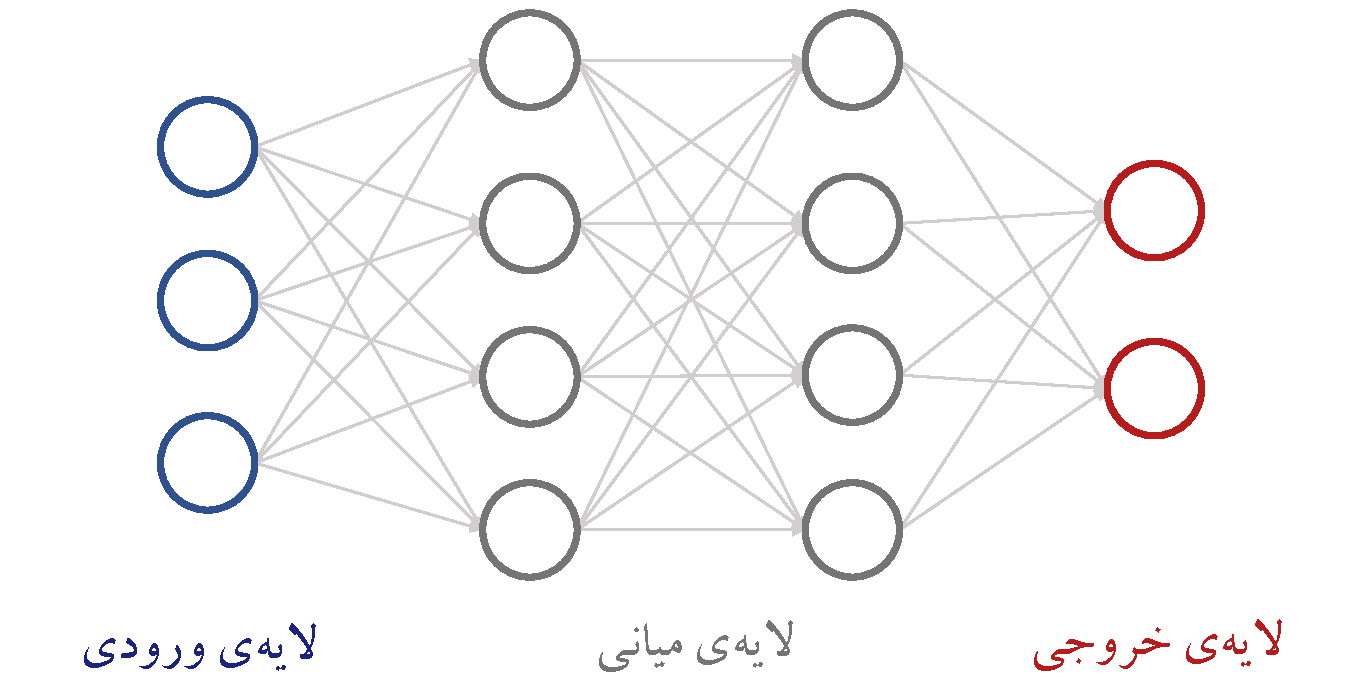
\includegraphics[scale=0.4]{Figures/neuralnet.pdf}
 	\caption[شبکه‌ی عصبی تماماً متصل با دو لایه‌ی میانی]{شبکه‌ی عصبی تماماً متصل با دو لایه‌ی میانی. هرکدام از لایه‌های ورودی، میانی و خروجی با رنگ یکتا  متمایز شده‌اند.}
 	\label{Fig:MLP}
 \end{figure}



\section{شبکه‌ی عصبی بازگشتی}
شبکه‌ی عصبی بازگشتی نوعی شبکه‌ی عصبی است که اتصالات میان گره‌های آن، حلقه تشکیل می‌دهند. درواقع، گره‌ها به نحوی به هم متصل هستند که به شبکه امکان به خاطر سپردن ورودی‌های گذشته را می‌دهد. به خاطر سپردن، این امکان را برای شبکه محیا می‌کند که تصمیمات آینده‌ی آن، وابسته به ورودی‌های پیشین نیز بشود \cite{rnn}. بدین ترتیب، خروجی شبکه می‌تواند حاصل ترتیبی از رویدادها باشد که در قالب بردار درآمده‌اند. از این رو، ورودی‌های یک شبکه‌ی عصبی بازگشتی، بصورت ترتیبی است. به عبارت دیگر ترتیب ورودی، خود دارای معنا و مفهوم است و باید ضمن دادن ورودی‌ها به شبکه، این مفهوم حفظ شود. بطور مثال جریان صدا، فریم‌های تصویر(فیلم)، و متن زبان طبیعی می‌توانند از شبکه‌های عصبی بازگشتی بهره ببرند. به این نوع ورودی‌ها، سری‌های زمانی\LTRfootnote{Time Series} نیز می‌گویند.
 \begin{figure}[!htb]
	\centering
	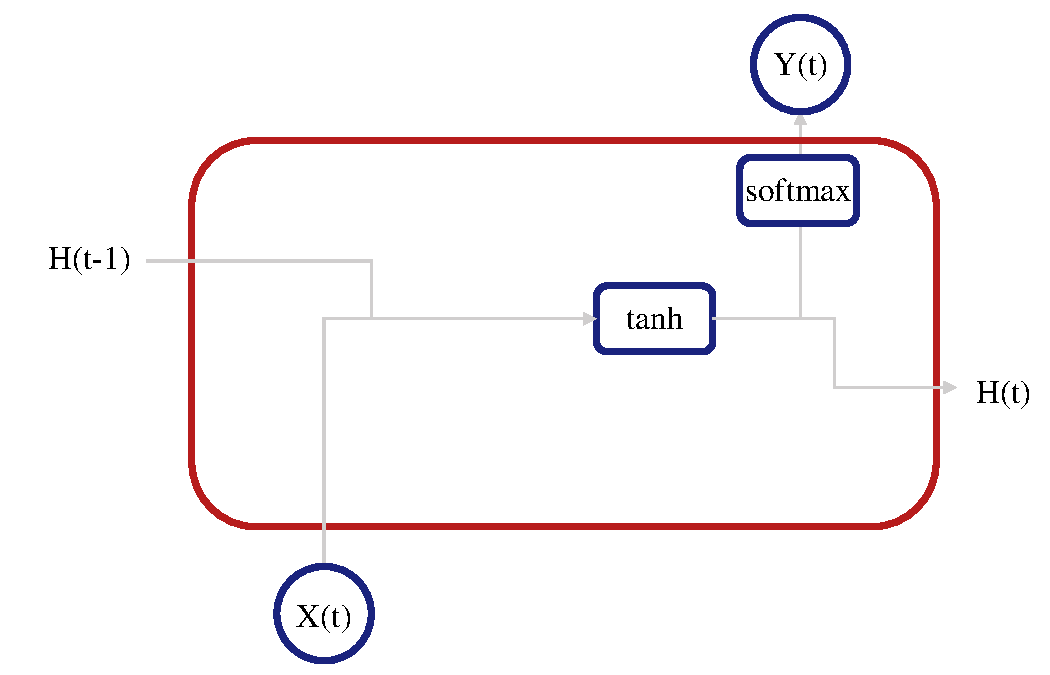
\includegraphics[scale=0.6]{Figures/RNN.pdf}
	\caption{یک بلوک از شبکه‌ی عصبی بازگشتی}
	\label{Fig:RNNBlock}
\end{figure}

شکل \ref{Fig:RNNBlock} معماری شبکه‌ی عصبی بازگشتی را نمایش می‌دهد. در معماری این نوع شبکه‌ها، علاوه بر بردار ورودی شبکه $X_{(i)}$، بردار حالت مخفی\LTRfootnote{ُHidden State} $H_{(i-1)}$  از مرحله‌ی قبلی شبکه نیز به عنوان ورودی به آن داده می‌شود. برای ورودی شبکه، وزن‌های بردار ورودی $W_{x}$ و برای بردار حالت مخفی، وزن‌های بردار حالت مخفی $W_{h}$، جداگانه در نظر گرفته می‌شود. بدین ترتیب، بردار حالت مخفی هر مرحله از طریق معادله‌ی \ref{Eq:RNNBlockHidden} و بردار خروجی از طریق معادله‌ی \ref{Eq:RNNBlockOutput} محاسبه می‌شود.
\begin{equation}
	H_{t} = tanh(W_{x}.X(t) + W_{h}.X(t-1) + b_{h})
	\label{Eq:RNNBlockHidden}
\end{equation}\vspace{-\baselineskip}
\begin{equation}
	Y_{t} = softmax(W_{Y}.H_{t} + b_{Y})
	\label{Eq:RNNBlockOutput}
\end{equation}
در معادلات فوق، $W_{Y}, W_{H}, b_{h}, b_{Y}$ همگی پارامترهای قابل آموزش هستند.


 \begin{figure}[!htb]
	\centering
	\includegraphics[scale=0.7]{Figures/RNNenrolled.pdf}
	\caption[شبکه‌ی عصبی بازگشتی گسترده شده در بعد زمان]{شبکه‌ی عصبی بازگشتی گسترده شده در بعد زمان. در این شکل هر بلوک بیانگر یک گام زمانی است.}
	\label{Fig:RNNenrolled}
\end{figure}
برای استفاده از شبکه‌ی عصبی بازگشتی در کاربرد پردازش متن، مطابق شکل \ref{Fig:RNNenrolled}، در هر گام زمانی\LTRfootnote{Time-Step}، یک واژه به همراه بردار حالت مخفی قبل به شبکه داده می‌شود. بردار تولید شده‌ی $Y_{(t)}$ به عنوان خروجی شبکه در گام زمانی $t$ و بردار $H_{(t)}$ به عنوان بردار حالت مخفی به گام زمانی بعد داده می‌شود. با چنین ساختار شبکه‌ای، می‌توان ورودی با طول پویا به شبکه داد.


برای استفاده‌ی شبکه‌ی عصبی بازگشتی در وظیفه‌هایی مانند ترجمه، عموماً از معماری رمزنگار - رمزگشا استفاده می‌کنند. در رمزنگار، ورودی شبکه‌ی عصبی تبدیل به یک بردار می‌شود. این بردار در گام بعد، وارد رمزگشا می‌شود تا نشانه‌های مورد نظر را تولید کند. شکل \ref{Fig:RNNenrolled}، مورد استفاده‌ی شبکه‌ی عصبی بازگشتی در رمزنگار را توضیح می‌دهد. شکل \ref{Fig:RNNdecoderenrolled} شیوه‌ی استفاده از شبکه عصبی بازگشتی در رمزگشا را به تصویر می‌کشد. در بخش رمزگشا، از آنجایی که نشانه‌های صحیح موجود نیست، نشانه‌ای قراردادی مانند $(BOS)$\LTRfootnote{Beggining of Sentence} را به عنوان اولین نشانه وارد شبکه می‌کنند. سپس در هر گام زمانی، نشانه‌ی تولید شده توسط مدل به عنوان ورودی مرحله‌ی بعد استفاده می‌شود. این کار تا زمانی تکرار می‌شود که نشانه‌ای قراردادی مانند $(EOS)$\LTRfootnote{End Of Sentence} تولید شود.
 \begin{figure}[!htb]
	\centering
	\includegraphics[scale=0.7]{Figures/RNNdecoderenrolled.pdf}
	\caption[شبکه‌ی عصبی بازگشتی در نقش رمزگشا، گسترده شده در بعد زمان]{شبکه‌ی عصبی بازگشتی در نقش رمزگشا، گسترده شده در بعد زمان. در این شکل هر بلوک بیانگر یک گام زمانی است.}
	\label{Fig:RNNdecoderenrolled}
\end{figure}

یک شبکه عصبی بازگشتی از نظر تئوری باید قادر به تولید دنباله‌هایی با هر پیچیدگی ای باشد اما در عمل مشاهده می‌کنیم که اگر تعداد گام زمانی در چنین شبکه‌ای به اندازه کافی زیاد باشد، در ذخیره سازی اطلاعات مرتبط با ورودی‌های قبلی به مدت طولانی ناتوان است \cite{RNNGradientProblem}.
علاوه بر اینکه این خصیصه توانایی شبکه را در مدل سازی ورودی‌های طولانی تضعیف می‌کند، باعث می‌شود که شبکه در زمان تولید دنباله‌ای از کلمات، در معرض ناپایداری قرار بگیرد. مشکلی که وجود دارد این است که اگر پیش‌بینی‌های شبکه تنها وابسته به چند ورودی اخیر باشد و این ورودی ها خود نیز توسط شبکه تولید شده باشند، شانس بسیار کمی برای تصحیح و جبران اشتباهات گذشته توسط شبکه وجود دارد. به طور مثال اگر ترجمه‌ی یک واژه در ابتدای جمله، به واژه‌ای در انتهای جمله وابسته باشد، و جمله‌ی یاد شده طولانی هم باشد، ممکن است شبکه نتواند به خوبی عمل کند. علت این امر دو مسئله‌ی گرادیان محو شونده\LTRfootnote{Vanishing Gradient} و گرادیان انفجاری\LTRfootnote{Exploding Gradient} است \cite{VanishingGradient}.
\\
انواع مختلفی از شبکه‌های عصبی بازگشتی وجود دارد؛ بطور مثال \lr{GRU} و \lr{LSTM} . از آنجا که در اکثر کاربرد‌های زبان طبیعی شبکه‌ی \lr{LSTM} مورد استفاده قرار می‌گیرد، تنها به معرفی این معماری پرداخته می‌شود.

\section{حافظه‌ی کوتاه‌مدت طولانی}
داشتن یک حافظه بلند مدت شبکه را به ثبات بیشتری می‌رساند؛ چراکه اگر شبکه بتواند از تاریخچه‌ی خود درک صحیحی پیدا کند، می‌تواند با مشاهده‌ی ورودی‌های ابتدایی، پیش‌بینی بهتری ارائه کند. شبکه‌ی حافظه‌ی کوتاه‌مدت طولانی\LTRfootnote{Long Short-Term Memory (LSTM)}، با معرفی سلول حافظه\LTRfootnote{Memory Cell} قادر است نسبت به حفظ حافظه فعلی از طریق دروازه‌های معرفی شده تصمیم‌گیری کند \cite{lstm}. ازنظر شهودی، اگر واحد \lr{LSTM} داده‌ی مهمی در دنباله ورودی را در گام‌های ابتدایی تشخیص دهد، با استفاده از دروازه‌های معرفی شده می‌تواند این اطلاعات را طی گام‌های زمانی بعدی نیز منتقل کند. بدین ترتیب، \lr{LSTM} می‌تواند این گونه وابستگی‌های بلندمدت را دریافت کرده و حفظ دارد. در ادامه به معرفی این دروازه‌ها پرداخته می‌شود.


 \begin{figure}[!htb]
	\centering
	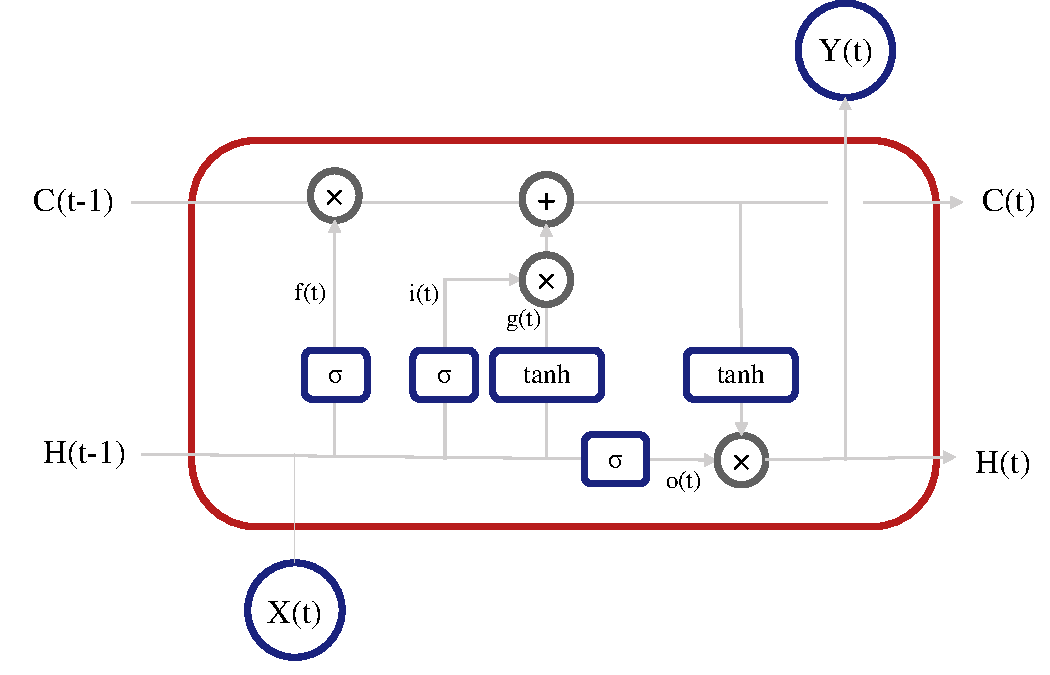
\includegraphics[scale=0.6]{Figures/LSTM.pdf}
	\caption{یک بلوک از حافظه کوتاه‌مدت طولانی}
	\label{Fig:LSTMBlock}
\end{figure}
شکل \ref{Fig:LSTMBlock} ساختار درون یک بلوک \lr{LSTM} را به‌تصویر می‌کشد. معماری \lr{LSTM}‌ دارای ۳ دروازه است؛ دروازه‌ی ورودی\LTRfootnote{Input Gate}، دروازه‌ی فراموشی\LTRfootnote{Forget Gate} و دروازه‌ی خروجی\LTRfootnote{Output Gate}.
این سه دروازه با همکاری یکدیگر حافظه‌ی فعلی سلول $C_{t}$ را بروزرسانی و حالت فعلی شبکه $H_{t}$ را تعیین می‌کنند.  
معادله‌ی \ref{Eq:LSTMForget} دروازه‌ی فراموشی $f_{t}$ را نشان می‌دهد. این دروازه مشخص می‌کند چه میزان از اطلاعات قبلی باید دور ریخته شود.
\begin{equation}
	f_{t} = σ(W_{f}.[H_{t-1},X_{t}] + b_{f})
	\label{Eq:LSTMForget}
\end{equation}
در این رابطه $σ$ تابع فعال ساز و $W$ و $b$ هردو پارامترهای قابل آموزش هستند. معادله‌ی \ref{Eq:LSTMInput} بیانگر دروازه‌ی ورودی است. این دروازه مشخص می‌کند چه میزان از اطلاعات ورودی در گام زمانی فعلی باید در حافظه‌ی فعلی سلول ذخیره شود.
\begin{equation}
	i_{t} = σ(W_{i}.[H_{t-1},X_{t}] + b_{i})
	\label{Eq:LSTMInput}
\end{equation}
معادله‌ی \ref{Eq:LSTMOutput} نشانگر دروازه‌ی خروجی است. دروازه‌ی خروجی مشخص می‌کند که با توجه به سلول حافظه $C_{t}$، چه چیزی در خروجی قرار گیرد.
\begin{equation}
	o_{t} = σ(W_{o}.[H_{t-1},X_{t}] + b_{o})
	\label{Eq:LSTMOutput}
\end{equation}
به همین ترتیب، حالت فعلی سلول حافظه ازطریق معادله‌ی \ref{Eq:LSTMCt} به دست می‌آید. در این معادله، $⊙$ بیانگر ضرب نقطه‌ای\LTRfootnote{Dot Product} است.
\begin{equation}
	\begin{array}{l}
		q_{t} = tanh(W_{q}.[H_{t-1},X_{t}] + b_{q})\\
		C_{t} = f_{t} ⊙ C_{t-1} + i_{t} ⊙ q_{t}
	\end{array}
	\label{Eq:LSTMCt}
\end{equation}
در آخر، حالت مخفی $H_{t}$ و خروجی $Y_{t}$ در زمان $t$، توسط معادله‌ی \ref{Eq:LSTMHt} محاسبه می‌شود.
\begin{equation}
	\begin{array}{l}
		H_{t} = o_{t} ⊙ tanh(C_{t})\\
		Y_{t} = softmax(H_{t}) 
	\end{array}
	\label{Eq:LSTMHt}
\end{equation}
\subsection{حافظه‌ی کوتاه‌مدت طولانی دوطرفه}
تا کنون، پیش‌فرض استفاده از \lr{LSTM} برای تعبیه‌ی کلمات به صورت ترتیبی و در یک جهت بود. اما در زبان طبیعی، وابستگی‌های معنایی دوطرفه هستند؛ به این معنا که تعبیه‌ی یک واژه می‌تواند علاوه بر وابستگی به واژه‌ی پیشین، به واژه‌ی بعد از خود نیز وابسته باشد. از این رو، بنظر می‌رسد که معماری اولیه‌ی \lr{LSTM} این نیاز را برطرف نمی‌کند. یکی از راهکارهایی که برای حل این مسئله ارائه کردند در شکل \ref{Fig:BILSTM} ترسیم شده است.


 \begin{figure}[!htb]
	\centering
	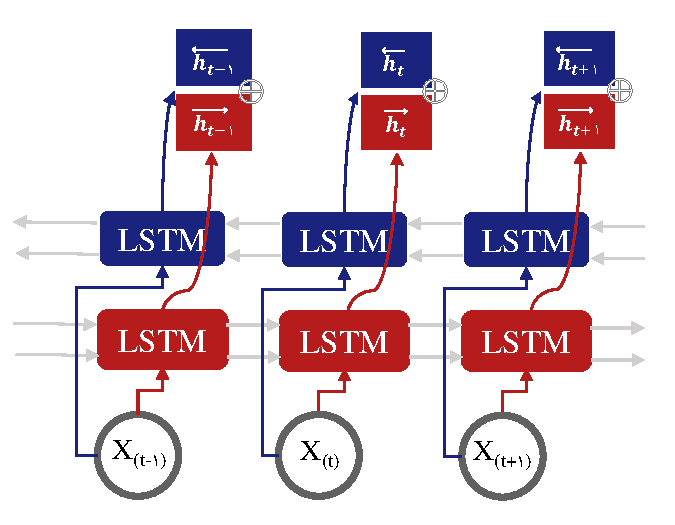
\includegraphics[scale=0.7]{Figures/bilstmenrolled.pdf}
	\caption[شبکه‌ی \lr{LSTM} دوطرفه]{شبکه‌ی \lr{LSTM} دوطرفه، گسترده شده در بعد زمان.}
	\label{Fig:BILSTM}
\end{figure}
شکل \ref{Fig:BILSTM}، یک \lr{LSTM} دوطرفه را نشان می‌دهد که در بعد زمان گسترده شده است. در \lr{LSTM} دوطرفه، یک لایه‌ی \lr{LSTM}، ابتدا از سمت چپ به راست $\overset{\rightarrow}{h}$، و سپس لایه‌ای دیگر از سمت راست به چپ $\overset{\leftarrow}{h}$، توالی واژه‌ها را پردازش می‌کند. تعبیه‌ی حاصل به دست آمده از این دو عملیات، با یکدیگر الحاق $\oplus$ می‌شوند تا تعبیه‌ی پایانی دوطرفه $(\overset{\rightarrow}{h}\oplus \overset{\leftarrow}{h})$ برای واژه ساخته شود.
\subsection{مکانیزم توجه}
روش دیگری که برای بهبود عملکرد شبکه‌ی \lr{LSTM} استفاده می‌شود، مکانیزم توجه \cite{attention_bahdanau} است. مکانیسم توجه به شبکه اجازه می‌دهد هنگام تصمیم گیری برای تولید هر نشانه، روی بخش‌های خاصی از ورودی تمرکز کند. این کار، با تخصیص وزن‌های مختلف به هر عنصر در دنباله ورودی انجام می شود. بدین ترتیب، مکانیزم توجه به عناصری که برای تصمیم گیری اهمیت بیشتری دارند وزن بیشتری می‌دهد. برداری که حاوی وزن‌ها است، بردار توجه نامیده می‌شود. این بردار توجه، به عنوان بخشی از ورودی، وارد شبکه‌ی \lr{LSTM} می‌شود. شیوه‌ی وارد کردن این بردار، الحاق آن با بردار تعبیه‌ی ورودی است. شکل \ref{Fig:attenbahdanau} شیوه‌ی محاسبه‌ی مکانیزم توجه را نشان می‌دهد.
 \begin{figure}[!htb]
	\centering
	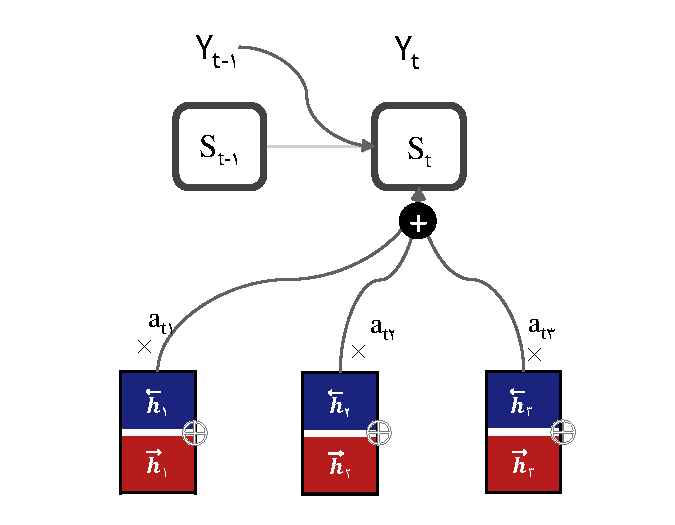
\includegraphics[scale=0.7]{Figures/bahdanauattention.pdf}
	\caption[مکانیزم توجه]{مکانیزم توجه تعریف شده در \cite{attention_bahdanau}.}
	\label{Fig:attenbahdanau}
\end{figure}


در واقع، در یک شبکه‌ی رمزگشای \lr{LSTM} که از مکانیزم توجه بهره می‌برد، حالت مخفی در هر مرحله‌ی زمانی، تابعی از حالت مخفی قبلی $S_{t-1}$، خروجی تولید شده‌ی قبلی $Y_{t-1}$ و بردار توجه $C_{t}$ است. این تابع را به صورت $s_{i}=f(S_{t-1},Y_{t-1},C_{t})$ نمایش می‌دهند. لازم به ذکر است که در این معادله، مقدار $C_{t}$ به ازاء هر واژه در خروجی متفاوت است. برای محاسبه‌ی $C_{t}$، جمع وزن‌داری از تمام حالت مخفی‌های رمزنگار ایجاد می‌شود، که وزن آن در طول فرایند یادگیری تغییر می‌کند. معادله‌ی \ref{Eq:atten_bahdanau} شیوه‌ی محاسبه‌ی $C_{t}$ را نمایش می‌دهد.
\begin{equation}
	c_{t}=\sum_{j=1}^{T_{x}}a_{tj}h_{j}
	\label{Eq:atten_bahdanau}
\end{equation}
در معادله‌ی \ref{Eq:atten_bahdanau}، $a_{tj}$ ماتریس متغیر قابل آموزش، به اندازه‌ی طول توالی ورودی $T_{x}$ در طول توالی خروجی $T_{y}$ است.
ماتریس توجه برای همه‌ی موقعیت‌ها، درواقع متغیر بوده و در طول فرایند آموزش مدل در وظیفه‌ی مورد نظر، تغییر می‌کند. از این رو، وزن‌های بردار توجه برای هر نوع وظیفه‌ی پردازش زبان طبیعی، متفاوت است.
\subsection{ضعف ذاتی}
با وجود برتری شبکه‌ی \lr{LSTM} در برابر شبکه‌ی بازگشتی، چالش‌هایی برای استفاده از این شبکه نیز وجود دارد. با توجه به این که پارامترهای شبکه‌ی \lr{LSTM}‌ نسبت به شبکه‌ی بازگشتی بسیار بیشتر است، آموزش آن و همگرا شدن شبکه نیازمند زمان و داده‌های بیشتری است. همچنین، \lr{LSTM} همیشه نمی‌تواند ظرافت‌های موجود در یک متن را درک کند. در ادامه، \lr{LSTM}‌ با وجود بهبود عملکرد شبکه‌ی بازگشتی، پوششی کوچک بر ضعف‌های ذاتی این نوع شبکه ایجاد کرده‌است \cite{info12110442}؛ اما ضعف ذاتی همچنان وجود دارد و نمی‌توان عملکردی مناسب در ترتیب‌های بزرگ دید \cite{VanishingGradient,Kag2020RNNs}. از طرف دیگر، به‌خاطر ورود ترتیبی بردارها به شبکه و پردازش سلسله مراتبی اطلاعات، نمی‌توان به خوبی از ظرفیت سخت‌افزارهای امروزی که قابلیت پردازش موازی و سریع داده‌ها را دارند بهره ‌برد. با توجه به مسائل ذکر شده، احتیاج به شبکه‌ای با پوشش واقعی این ضعف‌ها وجود دارد.
\section{شبکه‌ی عصبی کانولوشنی}

شبکه عصبی کانولوشنی\LTRfootnote{Convolutional Neural Network (CNN)} از یک لایه ورودی، لایه‌های پنهان و یک لایه خروجی تشکیل شده است. 
 در هر عملیات کانولشن، یک ماتریس هسته و یک ماتریس ورودی وجود دارد. ماتریس هسته\LTRfootnote{Kernel} که به آن فیلتر نیز می‌گویند، با حرکت روی ماتریس ورودی و ضرب نقطه‌ای مقادیر دو ماتریس که در معادله‌ی  \ref{Eq:Convolution} تعریف شده است، ماتریس خروجی را تولید می‌کند. به ماتریس تولید شده نقشه‌ی ویژگی\LTRfootnote{Feature Map} می‌گویند. 
 \begin{equation}
 	c=A\left(x\odot f+b\right)
 \label{Eq:Convolution} 
\end{equation}
در معادله‌ی فوق که عملیات کانولوشن را نشان می‌دهد، ورودی $x$، هسته $f$ و تابع فعال‌ساز $A$، و عملیات کانولوشن با $c$ برابر است.\\
حرکت هسته بر روی ماتریس ورودی می‌تواند همراه با پرش باشد، به این معنا که از محاسبه‌ی برخی از پنجره‌های ممکن صرف نظر شده و پنجره‌ی بعدی را محاسبه می‌شود. به پارامتر تعیین کننده‌ی پرش پنجره، گام\LTRfootnote{Stride} می‌گویند. در صورتی که از پد\LTRfootnote{Pad} استفاده نشود، ابعاد ماتریس ویژگی کوچک‌تر از ماتریس ورودی می‌شود. پد در شبکه‌ی کانولوشنی به معنای ایجاد موقعیت‌های جدید در ماتریس، با مقادیر ازپیش تعریف شده است. این مقادیر از پیش تعریف شده می‌تواند با توجه به سیاست خاصی از اعداد درون ماتریس انتخاب شود یا عدد مشخصی مانند صفر درون آن قرار گیرد. همچنین استفاده از گام بزرگتر از ۱ باعث کوچکی ماتریس ویژگی می‌شود. اندازه‌ی خروجی را می‌توان با استفاده از معادله‌ی \ref{Eq:ConvolutionDimension} محاسبه کرد. در این معادله، گام با $S$ اندازه‌ی ورودی با $N$، اندازه‌ی هسته با $M$، اندازه‌ی پد با $P$ و اندازه‌ی خروجی با $O$ مشخص شده است.
  \begin{equation}
 	O=\frac{N - \left(M-1\right)+P}{S}
 	\label{Eq:ConvolutionDimension} 
 \end{equation}
ورودی شبکه‌ی کانولوشنی می‌تواند به اندازه‌ی دلخواه بعد داشته باشد. برای هر بعد می‌توان با استفاده از معادله‌ی \ref{Eq:ConvolutionDimension}، اندازه‌ی خروجی را محاسبه کرد. شکل \ref{Fig:CNN} انجام عملیات کانولوشن یک هسته بر روی یک ماتریس را نمایش می‌دهد. برای سادگی در نمایش، کانال ورودی برابر ۱ در نظر گرفته شده است. لازم به ذکر است که کانال ورودی همواره با کانال هسته برابر است. در صورتی که کانال ورودی بزرگتر از ۱ باشد، مقدار هسته در هر کانال متفاوت با دیگری‌است.
 \begin{figure}[!htb]
	\centering
	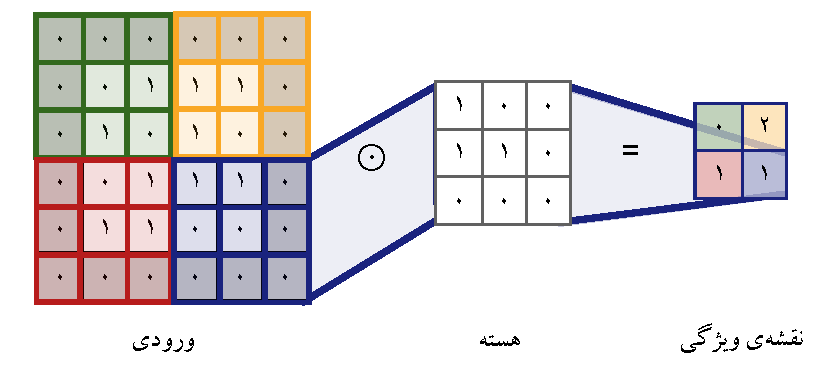
\includegraphics[scale=1]{Figures/cnn.pdf}
	\caption[کانولوشن یک هسته بر روی ماتریس ورودی]{
کانولوشن یک هسته بر روی ماتریس ورودی. در این شکل، هسته دارای طول ۳، عرض ۳ و کانال ۱ و ماتریس ورودی دارای طول ۳، عرض ۳ و کانال ورودی برابر۱ است. در این عملیات گام برابر با ۳ و پد برابر ۲ در نظر گرفته شده است. همچنین، رنگ خاکستری نمایانگر پد بوده و هر رنگ سبز، زرد، قرمز و آبی برابر با یک پنجره است.}
	\label{Fig:CNN}
\end{figure}

برای هر ورودی، یک بعد به عنوان تعداد کانال ورودی در نظر گرفته می‌شود. بعد از پایان اعمال یک هسته بر روی ورودی، آن بعد تبدیل به ۱ می‌شود. به عنوان مثال، در صورتی که ابعاد ورودی $(Height,Width,D)$ بوده، با فرض استفاده از پد، تعداد کانال ورودی برابر $D$، و و استفاده از یک هسته، خروجی برابر با $(Height,Width,1)$ می‌شود. اما عملیات کانولوشن می‌تواند با چند هسته و با مقادیر اولیه‌ی مختلف برای هسته‌ها تکرار شود. بدین ترتیب، در صورتی که از تعداد $K$ هسته استفاده شود، خروجی برابر با $(Heigh,Width,K)$ خواهد شد.
  در صورتی که شبکه‌ی کانولوشنی به صورت لایه‌ای باشد، نقشه‌ی ویژگی هر لایه، برای لایه‌ی مرحله‌ی بعد استفاده می‌شود. در لایه‌های بعد از لایه‌ی کانولوشن، معمولاً لایه‌های ادغامی\LTRfootnote{Pooling}، لایه‌های کاملاً متصل و لایه‌های نرمال‌سازی قرار می‌گیرند.
 \section{میدان تصادفی شرطی زنجیره‌ی خطی}
 میدان تصادفی شرطی\LTRfootnote{Conditional Random Field (CRF)}  زنجیره خطی، نوعی مدل گرافیکی احتمالی است که ابزار قدرتمندی برای مدل‌سازی و پیش‌بینی روابط بین متغیرها در یک دنباله می‌باشد. مانند سایر \lr{CRF}ها، \lr{CRF} زنجیره خطی هم، برای وظایف یادگیری با ناظر و هم بدون نظارت مانند طبقه بندی، تقسیم بندی\LTRfootnote{Segmentation} و برچسب گذاری استفاده می‌شود. \lr{CRF} زنجیره خطی، به ویژه برای کارهایی که شامل داده‌های متوالی هستند، مانند پردازش زبان طبیعی مفید است. اگرچه در هیچ کجای معماری پیشنهادی، از \lr{CRF}  استفاده نشده است، اما بخاطر به استفاده‌ی برخی از مدل‌های پیشین از آن، در این بخش به طور خلاصه معرفی می‌شود.
 
با در نظر گرفتن بردار خروجی رمزنگار برای وظیفه‌ی تشخیص جای خالی $Y=\{y_{1},y_{2},\cdots ,y_{N}\}$، توالی برچسب‌های جای خالی $s=\{s_{1},s_{2},\cdots ,s_{N}\}$ و تمام توالی‌های برچسب ممکن برای $s$ به عنوان $S(y)$، یک \lr{CRF} احتمال وقوع دنباله‌ی ترتیبی $s$ را در صورت مشاهده‌ی ورودی $y$، به ازای تمام $s$های ممکن، با معادله‌ی \ref{Eq:CRF} محاسبه می‌کند.
 \begin{equation}
 	p(s|y;W,b)=\frac{\prod_{i=1}^{N}e^{W^{T}_{s_{i-1},s_{i}}y_{i}+b_{s_{i-1},s_{i}}}}{\sum_{s^{\prime}\in S(y)}^{}\prod_{i=1}^{N}e^{W^{T}_{s^{\prime}_{i-1},s^{\prime}_{i}}y_{i}+b_{s^{\prime}_{i-1},s^{\prime}_{i}}}}
 	\label{Eq:CRF}
 \end{equation}

در معادله‌ی فوق، $W^{T}_{s_{i-1},s_{i}}$ بردار وزن و$b_{s_{i-1},s_{i}}$ بایاس متناظر با جفت برچسب $(s_{i},s_{i-1})$ است. همچنین، $W^{T}_{s^{\prime}_{i-1},s^{\prime}_{i}}$ بردار وزن و $b_{s^{\prime}_{i-1},s^{\prime}_{i}}$ بایاس متناظر با جفت برچسب $(s^{\prime}_{i},s^{\prime}_{i-1})$ هستند. معادله‌ی فوق، احتمال وقوع دنباله‌ی $s$ را در صورت مشاهده‌ی بردار تعبیه‌ی $y$ حساب می‌کند. برای انتخاب برچسب‌ها در \lr{CRF}، از الگوریتم \lr{Viterbi} استفاده می‌شود. معادله‌ی \ref{Eq:viterbi}،  محتمل‌ترین دنباله برچسب‌گذاری $s^{*}$ را محاسبه می‌کند.
 \begin{equation}
	s^{*}=	\underset{s\in S(y)}{argmax}  \: p(s|y; W,b)
	\label{Eq:viterbi}
\end{equation}

\section{ترنسفورمرها}
در سال‌های اخیر و با معرفی معماری ترنسفورمر\LTRfootnote{Transformer}، جهش قابل توجهی در عملکرد مدل‌های پردازش زبان طبیعی ایجاد شده است. معماری ترنسفورمر، آغازگر سبک جدیدی از طراحی شبکه‌ی عصبی است. این معماری‌ها، صرفاً با اتکاء بر مکانیزم توجه، داده‌های ترتیبی را تجزیه، تحلیل و پردازش می‌کنند \cite{transformerboom}. ترنسفورمر معایب شناخته‌شده‌ی شبکه‌های عصبی بازگشتی یعنی گرادیان محو شونده و گرادیان انفجاری را تا حد زیادی برطرف می‌کند. در گذشته، برای حفظ اطلاعات موجود در توالی، داده به صورت ترتیبی وارد شبکه می‌شد؛ اما در شبکه‌ی ترنسفورمر، با تکیه بر مکانیزم توجه، داده‌ها به صورت موازی و همزمان وارد شبکه می‌شوند. این امر باعث افزایش چشمگیر سرعت آموزش شبکه و همچنین استفاده‌ی بهینه از سخت‌افزارهای امروزی شده است.
 از طرف دیگر، برای پردازش دوطرفه‌ی متن در شبکه‌ی عصبی بازگشتی، جمله یک بار از راست به چپ و سپس از چپ به راست وارد شبکه شده و تعبیه‌ی خروجی با هم الحاق می‌شد. اگرچه اینکار مفید بود، اما تعبیه‌ی حقیقی دوطرفه از جمله ایجاد نمی‌کرد. اتکاء شبکه‌ی ترنسفورمر بر مکانیزم توجه، موجب ایجاد یک تعبیه‌ی دوطرفه‌ی حقیقی می‌شود؛ چراکه ترنسفورمر به صورت همزمان به تمام موقعیت‌های موجود درون جمله دسترسی دارد.
 
 
با توجه به استفاده‌ی گسترده‌ی مدل پیشنهادی از این معماری، در بخش پیش رو به تفصیل به معرفی معماری ترنسفورمر پرداخته می‌شود. ابتدا ایده‌ی کلی این معماری برای پردازش داده‌های ترتیبی تشریح شده و سپس اجزایی که این ایده را محقق می‌کنند، معرفی می‌شوند. در پایان، تغییراتی که داده در جریان گذر از این معماری به خود می‌بیند، به تفصیل توضیح داده می‌شود.


شکل \ref{Fig:Transformers}، معماری ترنسفورمر را نمایش می‌دهد. ساختار ترنسفورمر مبتنی بر سبک رمزنگار-رمزگشا است که در گذشته بصورت گسترده در وظیفه‌های پردازش زبان طبیعی مورد استفاده بوده است. این معماری بصورت پیش‌فرض برای وظیفه‌ی ترجمه کاربرد دارد. این معماری بصورت مؤلفه‌ای\LTRfootnote{Component} بوده و می‌توان هرکدام از رمزنگار یا رمزگشا را جداگانه مورد استفاده قرار داد.
 \begin{figure}[!htb]
	\centering
	\includegraphics[scale=0.62]{Figures/transformers.pdf}
	\caption[معماری شبکه‌ی ترنسفورمر]{معماری شبکه‌ی ترنسفورمر. سمت چپ معماری رمزنگار و سمت راست معماری رمزگشای ترنسفورمر را نمایش می‌دهد.}
	\label{Fig:Transformers}
\end{figure}
در ساختار ترنسفورمر، به‌جای ورود ترتیبی نشانه‌ها به شبکه، کل نشانه‌ها بصورت همزمان وارد شبکه می‌شوند. با توجه به اینکه رمزنگار ترنسفورمر ذاتاً یک شبکه خود همبسته\LTRfootnote{AutoRegressive} نیست، برای حفظ اطلاعات مهمی که در ترتیب داده موجود است، از تعبیه‌ی موقعیتی\LTRfootnote{Positional Encoding} استفاده شده است. ازطرف دیگر، برای درک روابط معنایی درون جمله، از مکانیزم توجه چند سر استفاده شده است. چند سر بودن مکانیزم توجه به مدل کمک می‌کند تعداد بیشتری از روابط درون جمله را درک کند.
%% منبع
\subsection{مکانیزم توجه چند سر}
هدف از تعریف مکانیزم توجه چند سر، اضافه کردن محتوای زمینه‌ای هر واژه از یک جمله، به هر واژه در جمله‌ی دیگر است. به عنوان مثال، فرض کنید دو جمله‌ی \lr{A} و  \lr{B} وجود دارند و هدف، اضافه کردن پیش زمینه‌ی جمله‌ی \lr{A} به جمله‌ی \lr{B} است. با استفاده از مکانیزم توجه، می‌توان بردار جدیدی به ازاء هر نشانه‌ی موجود در جمله‌ی \lr{B} ایجاد کرد که محتوای معنایی جمله‌ی \lr{A} را در بر دارد. مکانیزم توجه این کار را با اضافه کردن جمع وزن داری از تعبیه‌ی هر نشانه‌ی موجود در \lr{A} به تعبیه‌ی نشانه‌ی \lr{B} انجام می‌دهد؛ یعنی ابتدا یک جمع وزن‌دار از تعبیه‌ی نشانه‌های \lr{A} ایجاد کرده، آنها را با هم جمع می‌کند تا یک بردار به دست آید. بردار به دست آمده، بیانگر ارتباطات و مفاهیم به دست آمده از جمله‌ی \lr{A} است که به نشانه‌ی فعلی درحال پردازش در جمله‌ی \lr{B} مربوط می‌شود. این کار به ازاء تمام نشانه‌های موجود در \lr{B} انجام می‌شود، تا تمام این نشانه ها حاوی پیش زمینه‌ی مربوطه شوند. مطابق شکل \ref{Fig:Attention}، این بردار پیش‌زمینه، توسط سه بردار کلید\LTRfootnote{Key}، مقدار\LTRfootnote{Value} و پرسش\LTRfootnote{Query} ایجاد می‌شود. عموماً کلید و مقدار از جمله‌ی مبدأ (در مثال ذکر شده، جمله‌ی \lr{A}) و پرسش از جمله‌ی مقصد (در مثال بالا، جمله‌ی \lr{B}) ایجاد می‌شود.
\begin{figure}[!htb]
	\centering
	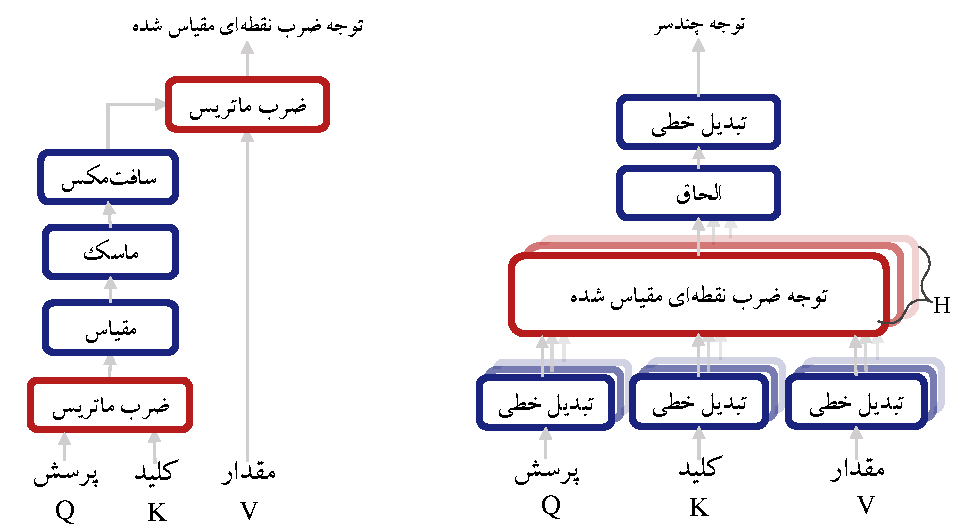
\includegraphics[scale=0.7]{Figures/attention.pdf}
	\caption[سمت چپ توجه ضرب نقطه‌ای مقیاس شده]{سمت چپ توجه ضرب نقطه‌ای مقیاس شده. سمت راست، توجه چندسر. در توجه چندسر، سرها به صورت موازی محاسبه می‌شوند.}
	\label{Fig:Attention}
\end{figure}


 معادله‌ی \ref{Eq:Attention}، نحوه‌ی محاسبه‌ی توجه ضرب نقطه‌ای مقیاس شده را نشان می‌دهد. با در نظر گرفتن $d_{k}$ به عنوان بعد بردار کلید و $d_{v}$ به عنوان بعد بردار مقدار در این معادله، کلید $K\in\mathbb{R}^{d_{k}}$، مقدار $V\in\mathbb{R}^{d_{v}}$، پرسش $Q\in\mathbb{R}^{d_{k}}$، عملیات ترانهادن\LTRfootnote{Transpose} $T$ و $.$ بیانگر ضرب ماتریس است. 
\begin{equation}
	Attention(Q, K, V) = V \times softmax(\frac{Q . K^{T}}{\sqrt{d_{k}}})
	\label{Eq:Attention}
\end{equation}
در مرجع \cite{transformer} نشان داده‌شده که برای مقادیر بزرگ $d_{k}$، مقادیر محصول نقطه‌ای بزرگ می‌شود که باعث شده تابع سافت‌مکس به نقطه‌ای برسد که گرادیان بسیار کوچکی دارد. برای مقابله با این اثر، آن‌ها با مقیاس $\frac{1}{\sqrt{d_{k}}}$ محصول نقطه‌ای را تغییر دادند؛ از این‌رو این معادله، ضرب نقطه‌ای مقیاس شده نام دارد.
\\
برای محاسبه‌ی توجه چند سر می‌توان از معادله‌ی \ref{Eq:MultiHead} استفاده کرد. در این معادله تعداد سرهای توجه $H$، و عملیات الحاق\LTRfootnote{Concatenation} با علامت $⊕$ مشخص شده است.
\begin{equation}
	\begin{array}{l}
		Attention_{h}(Q, K, V) = (Q . W_{h}^{Q}, K . W_{h}^{K}, V . W_{h}^{V}) \\
		Attention = Attention_{1} ⊕ Attention_{۲} ⊕ ... ⊕ Attention_{H} \\
		MultiHead = W^{M} . Attention
	\end{array}
	\label{Eq:MultiHead}
\end{equation}
در معادله‌ی \ref{Eq:MultiHead}، پیدا کردن روابط معنایی بین $H$ سر تقسیم شده‌اند. 
\\
درصورت تمایل برای جلوگیری از اعمال توجه بر روی برخی از موقعیت‌های درون جمله‌ی مبدا، می‌توان ماسک $M\in\mathbb{R}$ را در معادله‌ی \ref{Eq:Attention} اعمال کرد. در این صورت، معادله‌ی یاد شده به معادله‌ی \ref{Eq:MaskedAttention} تغییر می‌یابد.
\begin{equation}
	Attention_{Masked}(Q, K, V) = V \times softmax(\frac{Q . K^{T}}{\sqrt{d_{k}}}+M)
	\label{Eq:MaskedAttention}
\end{equation}
متعاقباً، مکانیزم توجه چند سر پوشیده، با معادله‌ی \ref{Eq:MaskedMultiHead} و با جابجایی مکانیزم توجه عادی با پوشیده بدست می‌آید. در این صورت، ماتریس ماسک $M_{diagonal}\in\mathbb{R}^{S\times T}$ نیز باید همراه با سایر ورودی‌ها، به تابع تغذیه شود؛ که در آن $S$ طول ترتیب مبدا و $T$ طول ترتیب مقصد است.
\begin{equation}
	\begin{array}{l}
		Attention^{h}_{masked}(Q, K, V) = (Q . W_{h}^{Q}, K . W_{h}^{K}, V . W_{h}^{V}) \\
		Attention_{masked} = Attention_{masked}^{1} ⊕ Attention_{masked}^{۲} ⊕ ... ⊕ Attention_{masked}^{H} \\
		MultiHead_{masked} = W^{M} . Attention_{masked}
	\end{array}
	\label{Eq:MaskedMultiHead}
\end{equation}
از مکانیزم توجه چند سر می‌توان برای مقاصد مختلف بهره برد. در ادامه به دو شیوه‌ی مرسوم آن و بینش پشت آن‌ها پرداخته می‌شود.
\subsubsection{توجه به خود}
زمانی که هر سه بردار کلید، مقدار و پرسش از یک جمله تولید شوند، به آن توجه به خود\LTRfootnote{Self-Attention} می‌گویند. هدف از معرفی توجه به خود، ایجاد تعبیه‌ی جدیدی برای نشانه است که در آن، تعبیه‌ی سایر نشانه‌های جمله دیده شده است. به عبارتی، به استفاده از توجه به خود، تعبیه‌ی نشانه‌ها با پیش‌زمینه‌ای که نشانه در آن استفاده شده آمیخته می‌شود.
\subsubsection{توجه متقابل}
در صورتی که کلید و مقدار از یک جمله و پرسش از جمله‌ی دیگری تولید شود، آن را توجه متقابل\LTRfootnote{Cross-Attention} می‌نامند. توجه متقابل کاربرد مهمی در وظیفه‌ی ترجمه دارد؛ چراکه با استفاده از آن، می‌توان ارتباطات معنایی میان دو جمله، در دو زبان مختلف را پیدا کرد.

\subsection{تعبیه‌ی موقعیتی}
به علت بازگشتی نبودن شبکه‌ی ترنسفورمر، باید روش دیگری برای حفظ ترتیب نشانه‌های ورودی معرفی شود. به این دلیل، در \cite{transformer} تعبیه‌ی موقعیتی را معرفی کرده‌اند. برای موقعیت نشانه‌های درون جمله، مطابق معادله \ref{Eq:PositionalEncoding} دو تابع تعریف شده است. در یک جمله، $N$ موقعیت مکانی (نشانه) و به ازاء هر نشانه، یک بردار $d_{model}$ بعدی\LTRfootnote{Dimension} وجود دارد.  معادله‌ی \ref{Eq:PositionalEncoding} برای بعدهای زوج از تابع سینوسی،‌ و برای بعدهای فرد تابع کسینوسی استفاده می‌کند. تعبیه‌ی موقعیتی، بعد یکسانی با بعد مدل $d_{model}$ دارد؛ به این منظور که بتوان تعبیه‌ی موقعیتی را با بردار تعبیه جمع کرد.
\begin{equation}
	\begin{array}{l}
		PE_(pos,2i) = Sin(\frac{pos}{10000^{\frac{2i}{d_{model}}}})\\\\
		PE_(pos,2i+1) = Cos(\frac{pos}{10000^{\frac{2i}{d_{model}}}})
	\end{array}
	\label{Eq:PositionalEncoding}
\end{equation}
در معادله‌ی بالا، موقعیت نشانه در جمله $pos$  و بعد مورد نظر آن  $i$  است. بدین ترتیب، برای بعد زوج و فرد هرکدام یک تابع وجود دارد. همچنین، طول موج‌های تولید شده یک افزایش هندسی از $2\pi$ به $2\pi . 10000$ می‌باشد. این توابع در مقایسه با توابعی که موقعیت مکانی را در طول آموزش یاد می‌گیرند، برتری دارند؛ چراکه می‌توانند در طول فرایند تست، تعبیه‌ی مکانی جملاتی با طول دیده نشده در فرایند آموزش را، در زمان تست استقرا کنند  \cite{transformer}.
\subsection{جریان داده}
در این بخش، تغییراتی که بر روی تعبیه‌ی اولیه‌ی نشانه‌ها صورت می‌گیرد تا به بردار نهائی تبدیل شود، تشریح می‌شوند. جریان داده به دو بخش زمان آموزش و زمان استنتاج\LTRfootnote{Inferrence} تقسیم می‌شوند. در ادامه، به توضیح این دو بخش پرداخته می‌شود.
\subsubsection{زمان آموزش}
به شکل \ref{Fig:Transformers} توجه کنید. در بخش رمزنگار، جمله‌ی ورودی ابتدا تبدیل به نشانه می‌شود. سپس برای این نشانه‌ها با استفاده از معادله‌ی \ref{Eq:PositionalEncoding} تعبیه‌ی موقعیتی ایجاد شده و با تعبیه‌ی اولیه نشانه‌ها جمع می‌شود. در مرحله‌ی بعد، ماتریس به دست آمده به صورت کامل و در یک مرحله وارد رمزنگار شده است؛ به این معنا که ورود ماتریس ترتیبی نیست. در بخش اول توجه به خود بر روی ماتریس ورودی ایجاد و سپس ماتریس توجه به دست آمده با ورودی جمع می‌شود. به عمل جمع کردن ماتریس توجه با ماتریس اولیه، اتصال باقی‌مانده\LTRfootnote{Residual Connection} می‌گویند \cite{residualconnection}. آخرین مرحله‌ی رمزنگار، یک شبکه‌ی تغذیه‌به‌جلو است که روی ماتریس حاصل از این شبکه نیز یک اتصال باقی‌مانده اعمال می‌شود.


در زمان آموزش، در بخش رمزگشا از شیوه‌ی اجبار معلم\LTRfootnote{Teacher Forcing} استفاده می‌شود. در این شیوه نشانه‌های هدف نیز همراه با ورودی به شبکه داده می‌شود. بدین ترتیب، به جای استفاده از خروجی شبکه برای تولید نشانه‌های احتمالی و آموزش ترتیبی مدل، فرایند آموزش را می‌توان به صورت موازی و بسیار سریع‌تر انجام داد. برای ورود نشانه‌های هدف در معماری رمزگشا، همه‌ی نشانه‌ها یک واحد به سمت راست جابجا می‌شوند؛ این کار به‌این منظور صورت می‌گیرد که شبکه بتواند در زمان استنتاج، که نشانه‌ی هدف را ندارد، با وارد کردن یک نشانه (معمولا $[BOS]$)، فرایند تولید نشانه را در رمزگشا آغاز کند. در گام نخست، ماتریس موقعیت مکانی با ماتریس تعبیه‌ی نشانه‌ها جمع شده و سپس وارد رمزگشا می‌شود. سپس عملیات توجه به خود چندسر پوشیده بر روی ماتریس تعبیه‌ی نشانه‌ها انجام و یک اتصال باقی‌مانده اعمال می‌شود. پوشیده در اینجا، به منظور استفاده از یک ماسک ماتریس مثلثی بالایی\LTRfootnote{Upper Triangular Matrix} است که از پردازش موقعیت‌های غیرمجاز توسط مکانیزم توجه جلوگیری می‌کند. این موقعیت‌های غیرمجاز در زمان آموزش، موقعیت‌های جلوتر از نشانه‌ی درحال پردازش هستند؛ چراکه کمک گرفتن از آن‌ها در زمان آموزش، برای مدل وابستگی ایجاد می‌کند، و از آن‌جا که در زمان استنتاج نشانه‌های موقعیت‌های جلوتر ناشناخته هستند، عملکرد مدل با اختلال روبرو می‌شود.
در گام دوم، کلید و مقدار از آخرین لایه‌ی رمزنگار، و پرسش از تعبیه‌ی نشانه‌ها، ایجاد و وارد واحد توجه متقابل می‌شود. در ادامه، ماتریس ایجاد شده از توجه متقابل با ماتریس تعبیه جمع، و وارد یک لایه‌ی تغذیه‌به‌جلو می‌شود. بر روی ماتریس حاصل از تغذیه‌به‌جلو نیز یک اتصال باقی‌مانده اعمال شده و بعد از یک لایه‌ی خطی و تابع سافت‌مکس، خروجی نهائی رمزگشای ترنسفورمر ایجاد می‌شود.

\subsubsection{زمان استنتاج}
تفاوت زمان استنتاج با آموزش در عدم وجود نشانه‌های هدف است؛ به همین دلیل، این تفاوت خود را در شیوه‌ی استفاده از رمزگشا نشان می‌دهد. در زمان استنتاج، رمزگشا تولید نشانه‌های خروجی را به صورت ترتیبی انجام می‌شود. بدین منظور، بعد از اتمام فرایند رمزنگاری، با دادن نشانه شروع $[BOS]$ به‌عنوان اولین نشانه به رمزگشا فرایند تولید خروجی آغاز می‌شود. سپس تمام فرایند‌های ذکرشده در زمان آموزش تکرار می‌شوند تا یک نشانه به عنوان خروجی تولید شود. خروجی تولید شده مجددا با نشانه‌ی $[BOS]$ الحاق شده و به عنوان ورودی مرحله بعد به رمزگشا تغذیه می‌شود. مراحل ذکر شده، تا رسیدن به نشانه‌ی $[EOS]$ تکرار می‌شوند.

\section{تعبیه‌ی نشانه‌ها}
برای این که جملات وارد شبکه‌ی عصبی شوند، باید ابتدا به واژه‌ها شکسته و واژه‌ها تبدیل به نشانه شوند. برای وارد کردن هر نشانه به شبکه، باید تعبیه‌ای از آن نشان وجود داشته باشد. تعبیه برداری از اعداد حقیقی است که بیانگر مفهوم آن نشانه در زبان طبیعی است. روش‌های تعبیه‌ی نشانه‌ها را می‌توان به دو گروه تقسیم نمود؛ تعبیه‌ی برداری ثابت و مدل‌های زبانی. در ادامه، این دو شیوه معرفی می‌شوند. 
\subsection{تعبیه‌ی برداری ثابت}
تعبیه برداری ثابت، نوعی از تعبیه است که در آن نمایش یک واژه یا عبارت معین از روی مجموعه‌ی متنی\LTRfootnote{Corpus} ایجاد می‌شود و در طول زمان تغییر نمی‌کند. پس از محاسبه‌ی تعبیه‌ی هر نشانه، فارغ از این ‌که نشانه در چه جمله‌ای استفاده شده باشد، تعبیه‌ی آن ثابت در نظر گرفته می‌شود. دو شیوه‌ی مطرح تعبیه‌ی برداری ثابت \lr{Word2Vec} و \lr{GloVe} هستند. در ادامه، به صورت خلاصه این دو تعبیه معرفی می‌شوند.
\subsubsection{\lr{Word2Vec}}
\lr{Word2Vec}
، مجموعه‌ای از مدل‌های شبیه به هم است که برای تعبیه‌ی واژه‌ها استفاده می‌شود. این مدل‌ها از شبکه‌ی تغذیه به جلوی کم‌عمق استفاده می‌کنند که برای بازسازی پیش‌زمینه‌ی زبانی واژه‌ها آموزش دیده‌اند. \lr{Word2Vec} مجموعه بزرگ متنی را به عنوان ورودی خود گرفته و یک فضای برداری با چند صد بعد تولید می‌کند. به هر واژه‌ی یکتا در مجموعه‌ی متنی، یک بردار متناظر در فضای برداری اختصاص داده می‌شود. \lr{Word2Vec} از دو روش برای تولید این بردارها بهره می‌برد؛ کیسه‌ی واژه‌های ممتد\LTRfootnote{Continuous bag-of-words} و اسکیپ‌گرام ممتد\LTRfootnote{Continuous Skip-Gram}. در هر دو روش،‌ یک پنجره لغزان\LTRfootnote{Sliding Window} از واژه‌های پیش‌زمینه، حول یک واژه‌ی اصلی در نظر گرفته می‌شود و به ازاء تمام واژه‌های موجود در مجموعه‌ی متنی عملیات محاسبه تکرار می‌شود. در روش کیسه‌ی واژه‌ها، مدل واژه‌ی اصلی را با استفاده از واژه‌های پیش‌زمینه‌ی موجود در پنجره حدس می‌زند. در این روش، ترتیب واژه‌های پیش‌زمینه تفاوتی ندارد. در روش اسکیپ‌گرام، مدل با گرفتن واژه‌ی اصلی، واژه‌های پیش‌زمینه‌ی آن را پیش‌بینی می‌کند. در این روش، واژه‌هایی که در پنجره ازنظر فاصله به واژه‌ی اصلی نزدیک‌تر هستند وزن بیشتری دارند. نویسندگان \lr{Word2Vec} اظهار کرده‌اند که کیسه‌ی واژه‌ها سرعت بیشتری دارد و در مقابل عملکرد اسکیپ‌گرام در مواجه با واژه‌های کمیاب بهتر است \cite{word2vec}.
\subsubsection{\lr{GloVe}}
\lr{GloVe} 
از شبکه‌ی عصبی استفاده نمی‌کند. در این شیوه‌ی تعبیه، ابتدا یک مجموعه‌ی متنی بزرگ پیمایش و ماتریس هم‌آیی واژه‌ها\LTRfootnote{Word Co-occurance Matrix} تشکیل می‌شود. سپس با این فرض که محصول نقطه‌ای بردار تعبیه‌ی دو واژه که در ماتریس هم‌آیی موجود هستند،  باید با تعداد هم‌آیی آن دو واژه رابطه داشته باشد، تعبیه‌ی واژه‌ها را در فضای برداری شکل می‌دهد \cite{glove}.
\subsection{مدل‌های زبانی}
نقص اصلی تعبیه برداری ثابت، این است که قادر به درک پیش‌زمینه‌ی مربوط به واژه نیست. این مشکل، عملکرد آن را برای پیش‌بینی دقیق معنای جمله و همچنین تولید متن محدود می‌کند. علاوه بر این، تعبیه‌های تولید شده ثابت‌اند؛ به این معنی که پس از پایان فرایند آموزش، نمی‌توان آنها را برای کاربر خاص بهینه یا با واژه‌های جدید که وارد زبان می‌شوند سازگار کرد.
یک مدل زبانی\LTRfootnote{Language Model} نسبت به زمینه کلام آگاه است؛ یعنی معنای جمله‌ای که واژه در آن‌ها آمده را درک می‌کند. این ویژگی باعث شده مدل زبانی قدرت پیش‌بینی دقیق‌تری داشته باشد. از این‌رو، یک مدل زبانی با دیدن یک جمله و در چالش حدس زدن یک جای خالی، می‌تواند واژه‌های مناسب تری را برای آن جای خالی پیشنهاد کند. در واقع، هدف اصلی مدل زبانی، محاسبه‌ی احتمال وقوع یک واژه، درون یک جمله است. به عنوان مثال، اگر عبارت "من قصد خواندن یک..." به مدل زبانی داده شود، مدل احتمال وقوع "کتاب" در ادامه‌ی این جمله را بیشتر از "خودرو" در نظر می‌گیرد. از طرف دیگر، تعبیه‌ی واژه‌ها در مدل زبانی، یک بردار ثابت نیست؛ بلکه تابعی است از سایر واژه‌هایی که در جمله حضور دارند. آموزش مدل‌های زبانی معمولا کاری هزینه‌بر و گران است. معمولا در فرایند آموزش آن‌ها، یک یا چند وظیفه بر روی حجم زیادی از داده‌های متنی تعریف می‌شود.
 \\ 
 در ادامه، ‌به معرفی دو مدل زبانی اِلمو که مبتنی بر \lr{LSTM} و بِرت که مبتنی بر ترنسفورمر است پرداخته می‌شود.
\subsubsection{المو}
\begin{figure}[!htb]
	\centering
	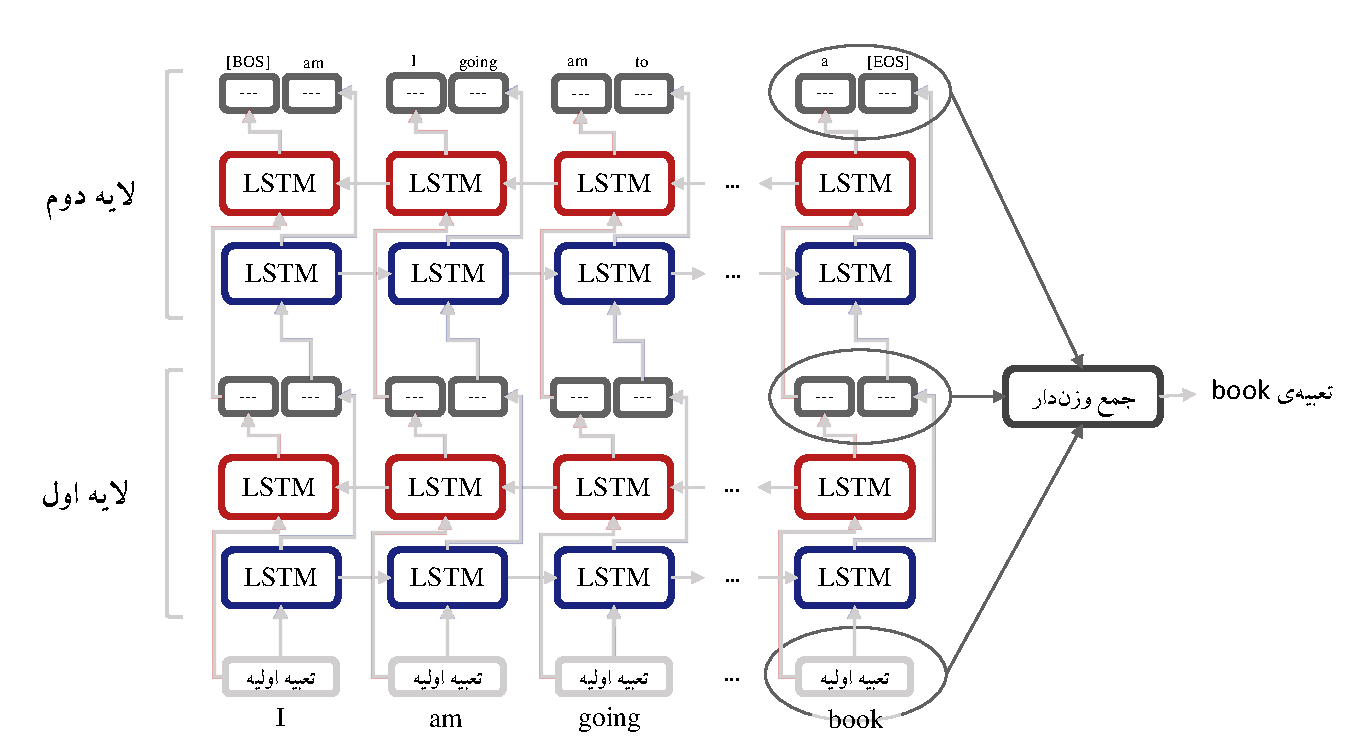
\includegraphics[scale=0.65]{Figures/elmo.pdf}
	\caption[معماری مدل زبانی المو]{معماری مدل زبانی المو. ورودی شبکه \lr{"I am going to read a book"} است. رنگ آبی برای  تعبیه‌ی چپ به راست و رنگ قرمز برای راست به چپ اختصاص دارد. برای جلوگیری از پیچیدگی شکل، اتصال باقی‌مانده در این شکل رسم نشده است.}
	\label{Fig:elmo}
\end{figure}
همانطور که گفته شد، برای ورود واژه‌ها به شبکه‌ی عصبی، باید واژه تبدیل به شناسه و شناسه تبدیل به بردار شود. در اِلمو \LTRfootnote{ELMo: Embedding From Language Models}، برای ایجاد بردار اولیه‌ی نشانه، از تعبیه‌ی الفبایی\LTRfootnote{Character Embedding} استفاده می‌شود. بدین منظور، ابتدا واژه به سطح الفبا شکسته شده، برای هر حرف الفبا یک شناسه‌ی یکتا، و برای هر شناسه یک بردار در نظر گرفته می‌شود. در مرحله‌ی بعد، مجموعه تعبیه‌ی الفبای واژه وارد شبکه‌ی کانولوشنی با اندازه هسته‌ی گوناگون می‌شود. مدل اصلی المو از هسته‌هایی با اندازه‌های ۱ تا ۷، با کانال‌های 32، 32، 64، 128، 256، 512 و 1024 استفاده می‌کند. خروجی‌های هر لایه کانولوشن پس از آن \lr{Max-Pool} شده و به هم الحاق می‌شوند تا برداری با تعداد بعد 2048 را بسازند. این خروجی به عنوان تعبیه‌ی اولیه واژه در نظر گرفته می‌شود تا مطابق شکل \ref{Fig:elmo} وارد شبکه‌ی \lr{LSTM} شود. المو در ساختار شبکه‌ی خود از \lr{LSTM} در دو جهت و به صورت دو لایه استفاده می‌کند. باید توجه داشت که ساختار شبکه با دو لایه‌ی \lr{Bi-LSTM} متفاوت است، چراکه ابتدا دو لایه متن را از چپ به راست و دو لایه را از راست به چپ پردازش می‌کند. در لایه‌ی چپ به راست،  در هر گام زمانی، وظیفه‌ی \lr{LSTM}‌ حدس زدن واژه‌ی بعدی، و در لایه‌ی راست به چپ، وظیفه‌ی آن حدس زدن واژه‌ی پیشین است. میان تعبیه‌ی اولیه و خروجی لایه‌ی اول، یک اتصال باقی‌مانده اضافه می‌شود. این عمل به مقاومت بیشتر شبکه درمقابل گرادیان محو شونده کمک می‌کند \cite{residualconnection}. در نهایت، برای تولید تعبیه‌ی پایانی، در هر لایه به صورت جداگانه، تعبیه‌ی چپ به راست با راست به چپ به یکدیگر الحاق می‌شوند. در پایان، جمع وزن‌دار میان تعبیه اولیه، خروجی الحاقی لایه‌ی اول و خروجی الحاقی لایه‌ی دوم را محاسبه می‌کنند. وزن‌های مربوط به این جمع وزن‌دار، برای هر وظیفه در پردازش زبان طبیعی متفاوت است.\\ خروجی هر لایه‌ی المو معنا و کاربرد خاص خود را دارد. خروجی لایه‌ی اول، بیشتر درمورد صرف و نحو زبان و خروجی لایه‌ی دوم، مرتبط به معنای جمله و واژه‌ها است \cite{elmo}.

\subsubsection{برت}
\begin{figure}[!htb]
	\centering
	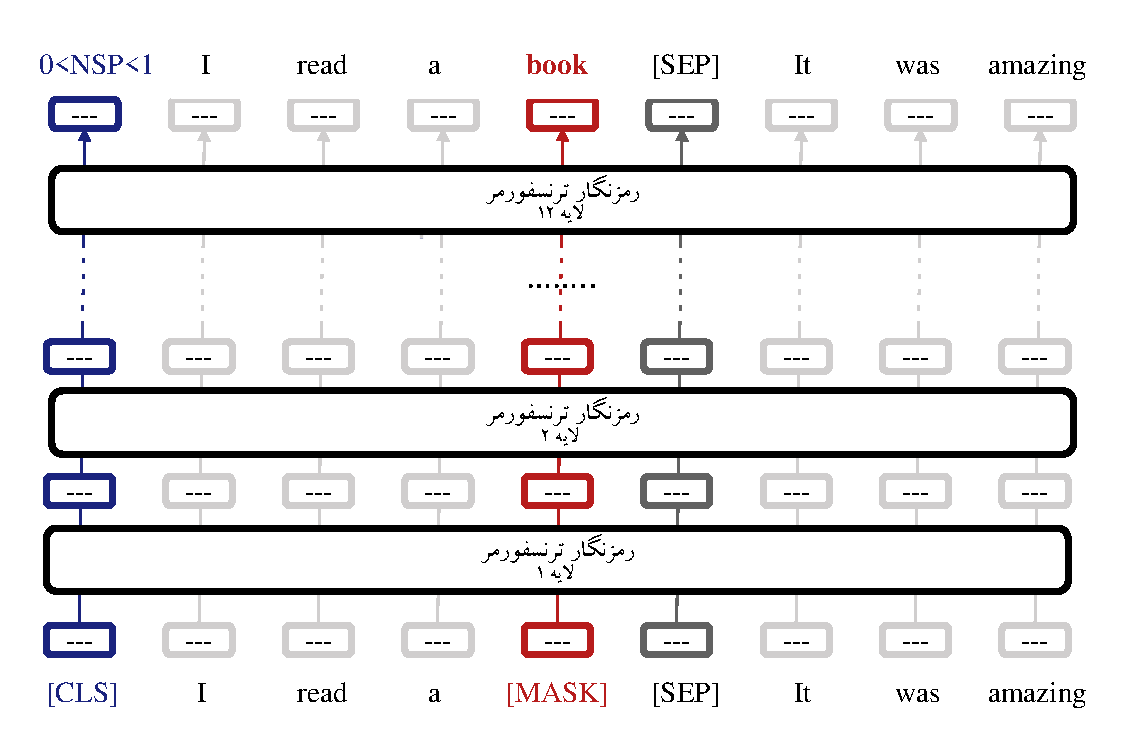
\includegraphics[scale=0.8]{Figures/bert.pdf}
	\caption[معماری مدل زبانی برت]{معماری مدل زبانی برت. ورودی شبکه دو جمله‌ی \lr{"I read a book. It was amazing"} است. واژه‌ی \lr{book} با استفاده از نشانه‌ی $[MASK]$ پوشیده شده است. این تصویر مربوط به نسخه‌ی $BERT_{base}$ می باشد.}
	\label{Fig:bert}
\end{figure}
بِرت\LTRfootnote{"Bert: Bidirectional Encoder Representations from Transformers"} 
یک مدل زبانی پیش‌آموز شده بر روی ترنسفورمرها است که برای استفاده در امور مختلف پردازش زبان طبیعی مورد استفاده قرار می‌گیرد \cite{bert}. با معرفی ترنسفورمرها \cite{transformer}، امکان ارائه یک تعبیه‌ی دوطرفه‌ی حقیقی فراهم شد. در \cite{bert} برای بهره‌گیری از قدرت ترنسفورمر، دو وظیفه‌ی خودناظر بر روی یک معماری لایه‌ای معرفی شده و ورودی‌ها به ترنسفورمر ساختارمند گردید. برای استفاده از برت، می‌توان مدل پیش‌آموز شده را دریافت کرد و با توجه به نیاز، آن را روی دیتاست مورد نظر تنظیم دقیق کرد. این شبکه در مدل پایه‌ی خود از ۱۲ لایه ترنسفورمر و در مدل بزرگ خود از ۲۴ لایه ترنسفورمر استفاده می‌کند. مدل برت در شکل \ref{Fig:bert} نمایش داده شده است.\\
  همانطور که بالا تلویحا گفته شد، برت در دو مرحله آموزش داده‌می‌شود؛ پیش‌آموزش\LTRfootnote{Pre-Training} و تنظیم دقیق\LTRfootnote{Fine-Tune}.\\
\textbf{پیش‌آموزش:}
 در این مرحله،‌ برت یاد می‌گیرد که زبان و پیش زمینه‌ی متن چیست. در مرحله پیش‌آموزش، مدل دو وظیفه‌ی متفاوت اما مرتبط را به صورت همزمان روی یک مجموعه متنی بدون برچسب یاد می‌گیرد. این دو وظیفه پیش‌بینی جمله‌ی بعد  و مدل‌سازی زبانی پوشیده هستند.\\
 الف) پیش‌بینی جمله‌ی بعد\LTRfootnote{Next Sentence Prediction (NSP)}: این وظیفه بر پایه‌ی این پیش‌فرض که دو جمله‌ی درون یک پاراگراف ازنظر معنایی به هم مرتبط هستند تعریف شده است. بر این اساس،  در وظیفه‌ی \lr{NSP}، برای دو جمله‌ی درون پاراگراف عدد ۱ و دو جمله‌ای که در یک پاراگراف نیستند عدد ۰ در نظر گرفته شده است. در این بخش، دو جمله‌ای که به مدل داده می‌شوند توسط نشانه‌ی $[SEP]$ از یکدیگر جدا شده‌اند. هدف مدل در این بخش تعیین ارتباط این دو جمله با یکدیگر است. نتیجه‌ی این تشخیص در اولین نشانه از خروجی (در شکل ‏\ref{Fig:bert} نشانه‌ی آبی رنگ) قرار دارد.\\
 ب) مدل‌سازی زبانی پوشیده\LTRfootnote{Masked Language Modeling (MLM)} : در این وظیفه مدل سعی می‌کند زمینه‌ی محتوایی متن را به صورت دوطرفه یاد بگیرد. به این منظور برخی واژه‌ها از جمله حذف شده و نشانه‌ی $[MASK]$ جای آن‌ها را می‌گیرد. سپس مدل سعی می‌کند با توجه به سایر واژه‌های موجود در جمله، جای خالی را با واژه‌ی مناسب پر کند. حذف واژه، با احتمال ۱۵ درصد روی تمام واژه‌های ورودی به جز واژه‌های کلیدی $[NSP]$ و $[SEP]$ صورت می‌گیرد.
 \\
\textbf{تنظیم دقیق:}
پس از مرحله‌ی پیش‌آموزش، برت زبان را یاد می‌گیرد اما نحوه‌ی استفاده از آن برای حل مسئله را بلد نیست. در مرحله‌ی تنظیم دقیق، مدل روش حل مسئله را آموزش می‌بیند. بدین منظور، با توجه به وظیفه‌ی مورد انتظار از مدل زبانی، نحوه‌ی آموزش مدل و ساختار رمزگشای آن مشخص می‌شود. به طور مثال می‌توان برای وظیفه‌ی پیش‌بینی احساسات، با قرار دادن یک شبکه‌ی تغذیه به جلو روی خروجی $[NSP]$ و آموزش مدل روی یک مجموعه داده‌ی پیش‌بینی احساسات، مدل را برای این وظیفه، تنظیم دقیق کرد. این کار نسبت به پیش‌آموزی، مدت زمان کمتری طول خواهد کشید؛ زیرا که شبکه به آموزش وزن‌های شبکه‌ی تغذیه به جلو که به تازگی اضافه شده‌اند می‌پردازد و بقیه‌ی پارامترهای مدل برت اندکی تغییر می‌کنند.
\section{جمع‌بندی}
در این فصل، ابتدا مفاهیم پایه‌ی این پایان‌نامه ذکر شد. سپس، مقدمه‌ای بر شبکه‌ی عصبی مطرح گردید. برای پردازش داده‌های ترتیبی، شبکه‌ی عصبی بازگشتی و \lr{LSTM} معرفی شدند. در ادامه، گفته شد که این نوع شبکه‌ها از مشکل گرادیان محو شونده رنج می‌برند. برای حل این مشکل مکانیزم توجه معرفی شد. اگرچه مکانیزم توجه مفید بود، اما اصل مسئله را حل نمی‌کرد. بنابراین، معماری ترنسفورمر معرفی گشت که از اساس ترتیبی نبوده و داده‌ها را به صورت همزمان وارد شبکه می‌کرد. همچنین، \lr{CRF} زنجیره خطی و شبکه‌ی عصبی کانولوشنی معرفی شدند. در پایان این فصل نیز، انواع تعبیه و مدل‌های زبانی معرفی گردیدند.
